\chapter{Introduction}
\label{chap:introduction}

This document serves to illustrate the \LaTeX{} template on the basis of the corporate design\index{Corporate Design} of the Bern University of Applied Sciences\index{Bern University of Applied Sciences} as well as a manual for its use. It is assumed that the user already has some experience with \LaTeX{} or is willing to familiarize with the subject. In the bibliography the user finds some useful information on \LaTeX{} on various books and documents on the Internet.

% Eintr�ge im Verzeichnis erscheinen lassen ohne hier eine Referenz einzuf�gen
\nocite{kopka:band1}
\nocite{raichle:bibtex_programmierung}
\nocite{MiKTeX}
\nocite{KOMA}
\nocite{TeXnicCenter}
\nocite{Marti06}
\nocite{Erbsland08}
\nocite{juergens:einfuehrung}
\nocite{juergens:fortgeschritten}

\section{Organising Documents}
\label{sec:einleitung_aufbau}

This document is structured according to the documentation of a project work or a thesis\index{thesis}. In Chapter \ref{chap:instructions}, the packages used are briefly explained, and instructions are given, how the bibliography and the glossary are to be used. Chapter \ref{chap:typeareatest} presents a sample chapter to audit the type area.

In figure \ref{fig:file_structure} the file structure is shown for this template.

\begin{figure}[H]
	\centering
		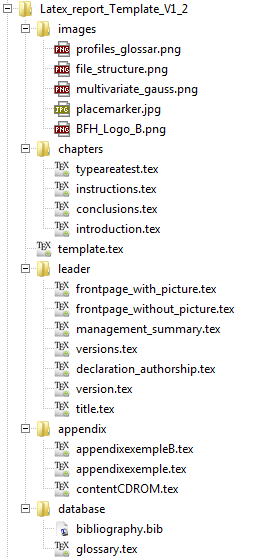
\includegraphics[scale=0.85]{images/file_structure.png}
	\caption{File structure}
	\label{fig:file_structure}
\end{figure}

\section{Contact}
\label{sec:introduction_contact}

The manufacturers of this template welcome any suggestions for improvement. Chapter \ref{sec:introduction_suggestions} shows possible suggestions for improvement\index{suggestions}.

\begin{table}[H]
	\centering
		\begin{tabular}{lll} \toprule
			\textbf{First Name Last Name} & \textbf{E-mail} & \textbf{Function} \\ \midrule
			Alfred Kaufmann & alfred.kaufmann@bfh.ch & Employer, Project Management, \\
			& & Supplements, Improvements \\ \midrule
			Fritz Dellsperger & Retired & Tips on the structure and layout \\ \midrule
			David Burri & Contracted out & First compilation of the Template \\ \bottomrule
		\end{tabular}
	\caption{Contact Persons}
	\label{tab:Contact Persons}
\end{table}


\section{Suggestions for Improvement}
\label{sec:introduction_suggestions}

\begin{itemize}
	\item Create a BFH Style Files
	\item Template for the Compilation of presentations with \LaTeX{}
\end{itemize}


